%%presentation.tex

\subsection{Présentation de l'entreprise \maxsea}
\textit{Maxsea International} est une entreprise (SAS) éditrice de
logiciels maritimes. Son produit phare "Maxsea Time Zero" est un
logiciel d'aide à la navigation maritime. Les bâtiments de son siège
social, à Bidart, sur la côte Basque, habritent une soixantaine
d'employés. La moitié sont des développeurs qui maintiennent le
logiciel, l'autre fait partie de la filiale \textit{MapMedia} qui
produit les cartes lisibles par le logiciel, ces derniers n'ont donc
pas de formation de développeurs.  Il existe deux autres filiales, une
en Espagne pour les relations commerciales et une de développeurs aux
États-Unis.


\subsection{Contacts: \maxsea}

%\subsubsection*{Entreprise : \maxsea}
\begin{itemize}
\item Adresse : Technopole Izarbel, 64210 Bidart – France
\item mail : info@maxsea.fr
\item tel : + 33 559 43 81 00
\item fax : + 33 559 43 81 01
\end{itemize}


\subsection{Description du stage}

\subsubsection*{Titre :} 
{\centering Migration d'une chaine de production cartographique
  vers un Cloud. \\}

\subsubsection*{Mots-clés :}
{\centering Cloud computing, Production cartographique, Windows Azure,
   Calcul parallèle, Géomatique. \\}

\subsubsection*{Sujet du stage :}
Dans le cadre de la production de données cartographiques vecteur, la
société \maxsea veut employer les technologies "Cloud" et en
particulier la solution "Azure" de \textit{Microsoft}. Pour cela, il
s’agira de coder des logiciels en $C\#$, s’appuyant sur le Framework
open source \textit{GDal/OGR}\,\footnote{\textit{Geospatial Data
    Abstraction Librairy} license by the \textit{Open Source
    Geospatial Foundation} (\textit{OSGeo})} (OGR pour le traitement
de données vecteur). Ceux-ci traiteront des étapes de la production de
données. Leur intérêt est la forte montée en charge possible dans le
Cloud, afin de réduire les temps de production (2 lots de production
par an, couvrant l’ensemble des cartes marines du globe).

\subsubsection*{Dates de stage :}
Le stage commence le 6 juin 2012 et finit le 21 septembre 2012.

\subsection{Acteurs du stage}
\subsubsection*{Maitre de Stage : Ronan GOLHEN}
\begin{itemize}
\item tel : + 33 614 17 65 05
\item mail : ronan.golhen@maxsea.fr
\end{itemize}


\subsubsection*{Tuteurs de stages}
\textbf{Arnaud CAPDEVIELLE}
\begin{itemize}
\item mail : arnaud.capdevielle@maxsea.fr 
\end{itemize}


\textbf{Arnaud REMY}
\begin{itemize}
\item mail : arnaud.remy@maxsea.fr
\end{itemize}



%\subsection{Enjeux et cahier des charges}
%le cahier des charges de son travail (en 5 pages maximum) :
%4 formats de cartes? Les prod mapmedia ne sont pas des dev

% - contexte qui décrit l'existant,
\subsection{Description de l'existant}
Pour produire ses cartes, la société \maxsea reçoit chaque année
diverses livraisons de cartes au format S57. Ses deux principaux
fournisseurs, \textit{Jeppesen} et \textit{Navionics}, livrent deux
fois par an l'ensemble des cartes maritimes du monde. Une seule de ces
livraisons contient 45000 fichiers. Au début du stage la chaine de
production des cartes au format dbv était localisée dans les locaux de
l'entreprise. Le temps de transformation était cependant préoccupant,
puisque les livraisons prenaient du retard. En effet, en utilisant les
12 serveurs disponibles pour cette opération de production ,quatre
mois étaient nécessaires au traitement d'une livraison.

La chaine de production de cartes vecteurs est supervisée par le
logiciel SSIS\,\footnote{SQL Server Integration Services} de
\textit{Microsoft}. Une fois les données reçues, par DVD ou
FTP\,\footnote{\textit{File Transfert Protocol}, Protocole de
  transfert de fichiers}, un opérateur lance l'exécution de
l'ETL\,\footnote{\textit{Extract Transform Load}, extraction
  transformation alimentation} SSIS. Celui-ci va lancer un par un les
différents traitements qui seront nécessaires à la
production. L'opérateur effectue différents contrôles plus ou moins
automatisés, notamment à la fin de la création du catalogue. Durant ce
processus les cartes sont manipulées sous forme de bases de données
spatiales. Les deux SGBD\,\footnote{\textit{Système de Gestion de Base
    de Données}} utilisées pour ces traitements sont SQL Server et
PostgresSQL. Les opérations sur celles-ci se font principalement via
FME\,\footnote{Logiciel propriétaire de SAFE SOFTWARE}, un ETL
Spatial, qui s'appuit sur le Framework open source spatial
\textit{GDal/OGR}.
%ici un schéma des étapes de production

% - description de la mission technique (travail à effectuer dans le
% contexte de l'étude)


\begin{figure}[h!]
  \caption{Captures d'écran du logiciel MaxSeaTZ.}
  \centering
    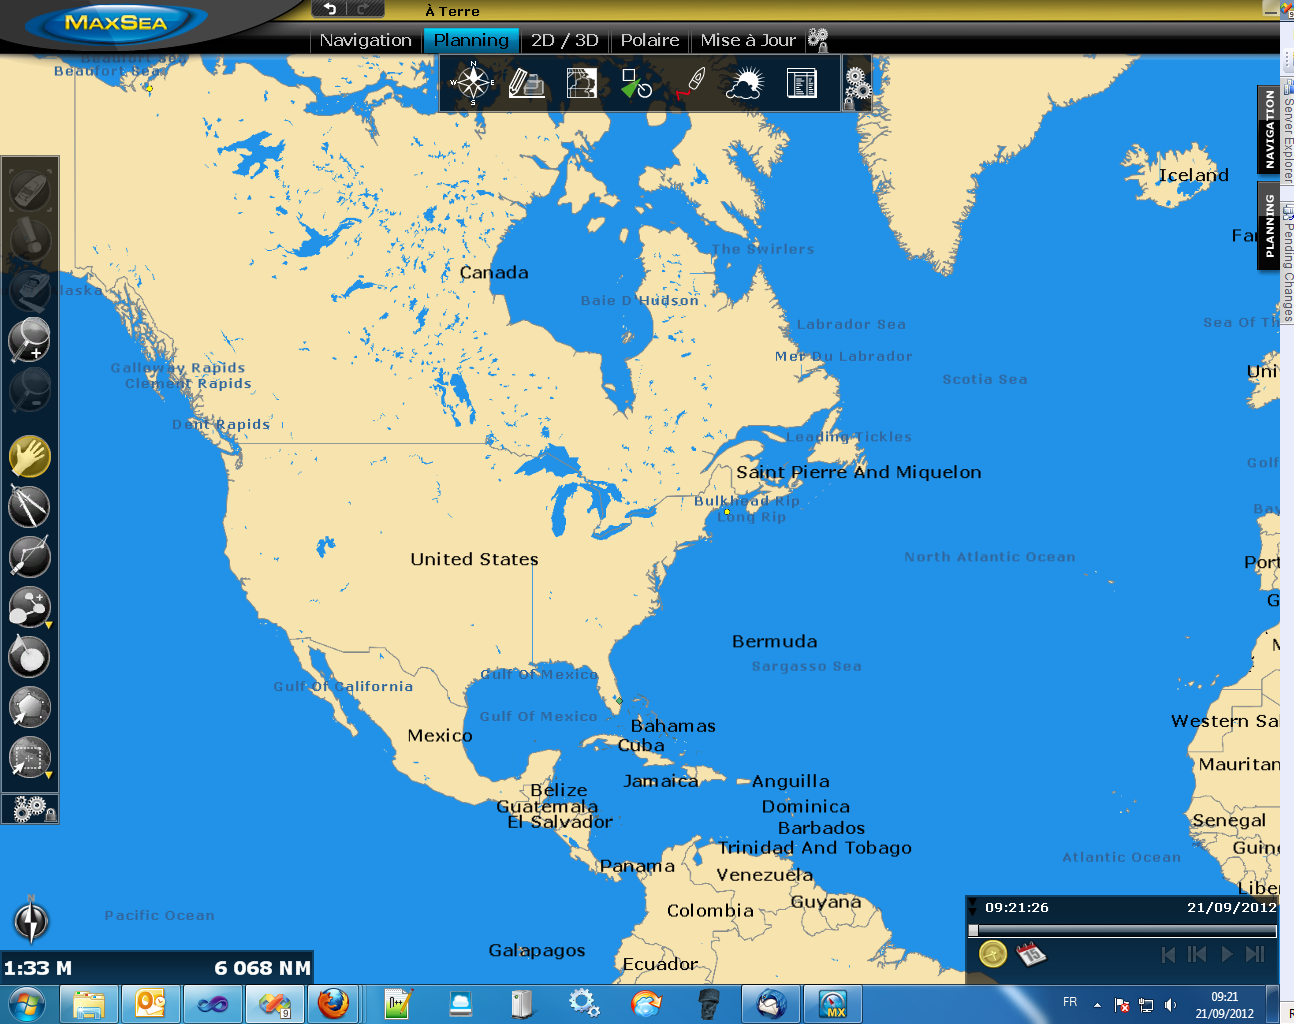
\includegraphics[width=0.45\textwidth]{images/MXTZ.png}
    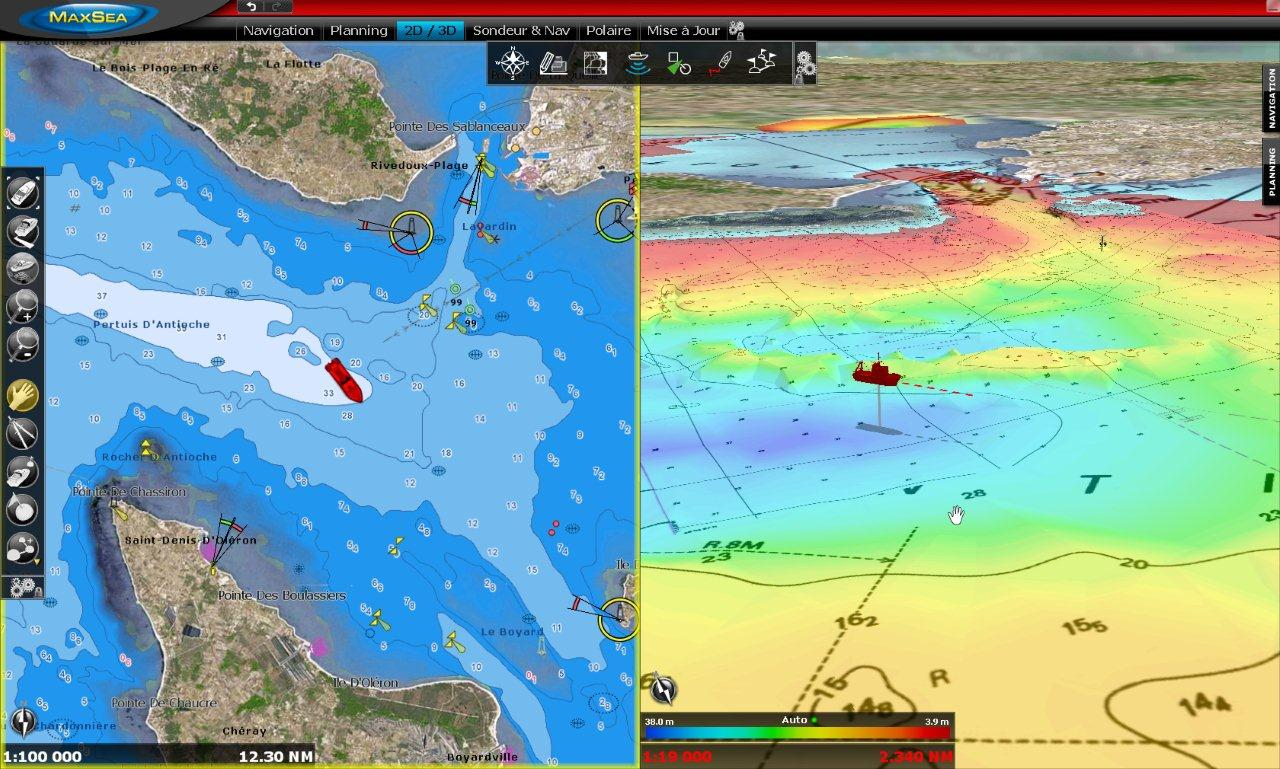
\includegraphics[width=0.45\textwidth]{images/MaxSeaTZ.jpg}
\end{figure}


\subsection{Mission Technique}
Le stage consiste à déployer la chaine de production dans un
environement de cloud computing. Ceci doit amener trois avantages à la
société. Le premier et le plus important est de pouvoir produire les
cartes dans le temps demandé. Ensuite vient la libération de
ressources machine au sein des locaux et la baisse du prix de revient
de la chaine de production vecteur.





